% CVPR 2022 Paper Template
% based on the CVPR template provided by Ming-Ming Cheng (https://github.com/MCG-NKU/CVPR_Template)
% modified and extended by Stefan Roth (stefan.roth@NOSPAMtu-darmstadt.de)

\documentclass[10pt,twocolumn,letterpaper]{article}

%%%%%%%%% PAPER TYPE  - PLEASE UPDATE FOR FINAL VERSION %%%%%%%%%
%\usepackage[review]{cvpr}      % To produce the REVIEW version
%\usepackage{cvpr}              % To produce the CAMERA-READY version
\usepackage[pagenumbers]{cvpr} % To force page numbers, e.g. for an arXiv version

% Include other packages here, before hyperref.
\usepackage{graphicx}
\usepackage{amsmath}
\usepackage{amssymb}
\usepackage{booktabs}
\usepackage{float}
\usepackage[table,xcdraw]{xcolor}
\usepackage{arydshln}


% It is strongly recommended to use hyperref, especially for the review version.
% hyperref with option pagebackref eases the reviewers' job.
% Please disable hyperref *only* if you encounter grave issues, e.g. with the
% file validation for the camera-ready version.
%
% If you comment hyperref and then uncomment it, you should delete
% ReviewTempalte.aux before re-running LaTeX.
% (Or just hit 'q' on the first LaTeX run, let it finish, and you
%  should be clear).
\usepackage[pagebackref,breaklinks,colorlinks]{hyperref}


% Support for easy cross-referencing
\usepackage[capitalize]{cleveref}
\crefname{section}{Sec.}{Secs.}
\Crefname{section}{Section}{Sections}
\Crefname{table}{Table}{Tables}
\crefname{table}{Tab.}{Tabs.}

\begin{document}

%%%%%%%%% TITLE - PLEASE UPDATE %%%%%%%%%
\title{VRDL HW1: Image Classification Report}

\author{Yi-Hsiang Ho, 111550106
% For a paper whose authors are all at the same institution,
% omit the following lines up until the closing ``}''.
% Additional authors and addresses can be added with ``\and'',
% just like the second author.
% To save space, use either the email address or home page, not both
% \and
% Second Author\\
% Institution2\\
% First line of institution2 address\\
% {\tt\small secondauthor@i2.org}
}
\maketitle

%%%%%%%%% BODY TEXT %%%%%%%%%
\section{Introduction}
\label{sec:intro}

The task is to classify creature images into 100 different categories using ResNet.
The core idea of my work is to leverage advanced data augmentation techniques,
MixUp and CutMix, and ensemble learning to improve the model's performance. ResNeXt
is chosen to be the backbone of the model. GitHub repository is available
at: 

%-------------------------------------------------------------------------
\subsection{ResNet}

ResNet (Residual Network) is a deep learning architecture introduced by Microsoft
in 2015 to address the vanishing gradient problem in very deep neural networks.
The main contribution is its residual block. It tries to learn the residual, or
difference, between layers by skip connections, which bypass one or more layers.
The method allows the network to learn identity mappings.

\subsection{ResNeXt}

ResNeXt is an improved variant of ResNet, introduced by Facebook AI in 2017,
which enhances performance by separating residual blocks into multiple small
branches. Instead of simply increasing depth or width, ResNeXt introduces the
concept of "cardinality," which refers to the number of parallel convolutional
paths in each residual block. This design improves feature learning while
maintaining computational efficiency.~\cite{Xie2016}

\begin{figure}[h]
  \centering
  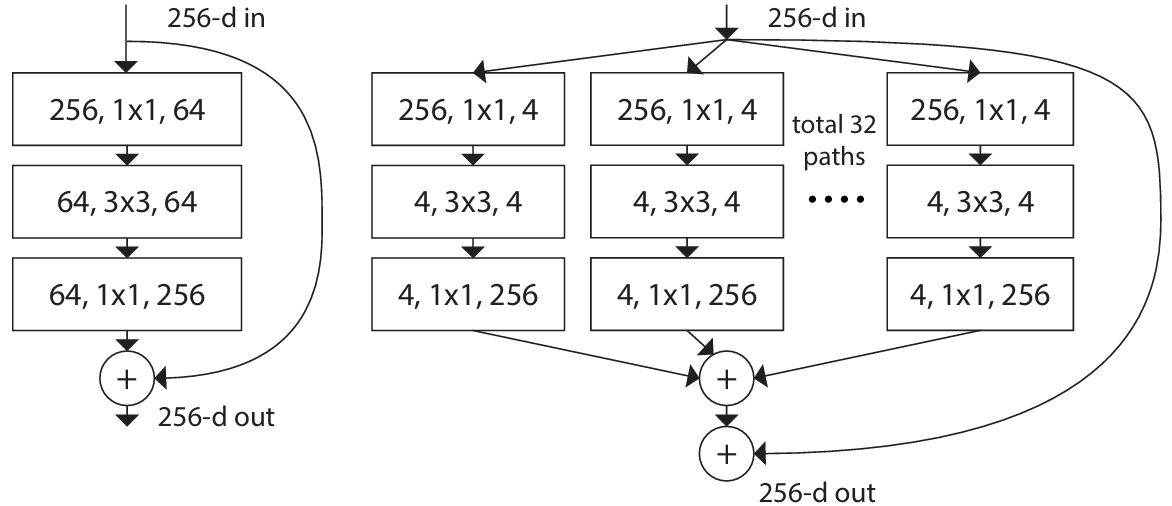
\includegraphics[width=0.8\linewidth]{assets/resnext_arch.png}
  \caption{\textbf{Comparison of ResNet and ResNeXt architecture.}
    Left: ResNet. Right: ResNeXt. Image source: \cite{Xie2016}.}
  \label{fig:resnext}
\end{figure}

\subsection{Mixup-Cutmix}

Mixup~\cite{zhang2018mixup} and CutMix~\cite{yun2019cutmix} are data
augmentation techniques that improve model generalization. Mixup blends
two images and their corresponding labels through linear interpolation,
while CutMix replaces
a region of one image with a patch from another and mix the labels. Both
methods enhance robustness, reduce overfitting, and improve classification
accuracy by promoting diverse feature learning.

\begin{figure}[h]
  \centering
  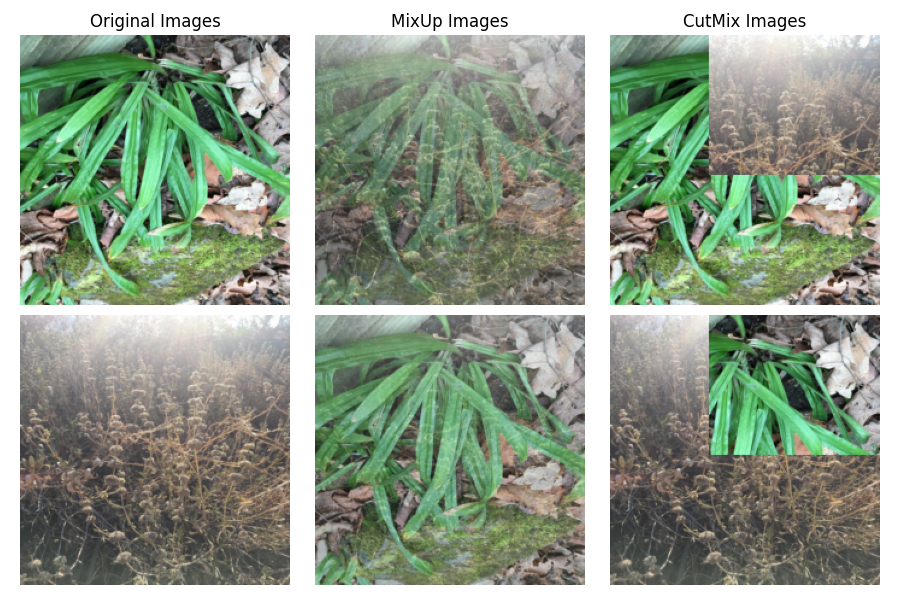
\includegraphics[width=0.8\linewidth]{assets/mixup_cutmix.png}
  \caption{\textbf{Visualization of Mixup and CutMix.}}
  \label{fig:mixup-cutmix}
\end{figure}

\subsection{K-fold Cross Validation \& Ensemble learning}

Cross-validation is a technique used to evaluate model performance by training
on different subsets of the data. It helps to reduce overfitting and improve
generalization. $K$-fold cross-validation divides the data into $K$ subsets, or
folds. The model is trained on $K-1$ folds and validated on the remaining fold.
This process is repeated $K$ times, with each fold serving as the validation set
once.

Ensemble learning combines multiple models to improve performance. It averages
the predictions of multiple models to make the final prediction. This technique
helps to reduce variance, increase accuracy, and improve model robustness.

\section{Method}
\label{sec:method}

\subsection{Data Pre-processing}

Data preprocessing plays a crucial role in the training pipeline. Basic
augmentations such as random horizontal flip and rotation are applied
before training. Random resized cropping is also added to both increase robustness
and meet the model's input requirements. Then, Mixup or CutMix is randomly chosen
as an additional data augmentation technique to improve the diversity of the training
dataset and smooth the labels. Note that no data augmentations are performed during
validation or testing. The only preprocessing in these period is
resizing to 224x224.

\subsection{K-fold and Test-Time Ensemble}

To further enhance model performance, I leverage the concept of $K$-fold. In
this work, I use $K$-fold to generate $K$ datasets, each with a different training
and validation set, and train $K$ sub-models on these datasets. In test-time ensemble,
I average the predictions of these $K$ sub-models to generate the final prediction. This
technique helps to improve generalization and enhance model performance.

\subsection{Model Architecture}

The model is built upon ResNeXt-101 64x4d, which has been pretrained on
ImageNet and the weights can be retrieved from PyTorch as
\verb'ResNeXt101_64X4D_Weights.IMAGENET1K_V1'. Also, to adapt the model to
this task, the final fully connected layer is modified to output predictions
for 100 classes.

\subsection{Optimization}

For optimization, AdamW is used with an initial learning rate of 1e-4. A
cosine annealing warm restart scheduler dynamically adjusts the learning
rate throughout training. Cross-entropy loss is employed as the loss
function, and training is performed with a batch size of 64 over 80 epochs.
Checkpoints are periodically saved, ensuring that the best-performing model
based on validation accuracy is retained.

\subsection{Hyperparameters}

\noindent The hyperparameter details are listed below:
\begin{itemize}
  \setlength\itemsep{0pt}
  \item Learning rate: 1e-4
  \item Optimizer: AdamW
  \item Scheduler: CosineAnnealingWarmRestarts
  \item Loss Function: CrossEntropyLoss
  \item Batch Size: 64
  \item Epochs: 80
  \item Number of Folds ($K$): 5
\end{itemize}

\section{Results}

In this section, I compare the performance of each component in the model.
The details of each method are listed:
\begin{itemize}
  \setlength\itemsep{0pt}
  \item ResNeXt: ResNeXt-101 64x4d pretrained on ImageNet.
  \item 5-Fold: Train ResNeXt on 5 different dataset seperated by 5-fold.
  \item Mixup \& Cutmix: ResNeXt with Mixup or CutMix data augmentation.
  \item All: Combines all the techniques mentioned in \cref{sec:method}.
\end{itemize}

The results are shown in \cref{tab:result}. All the results here are evaluated
by choosing the best checkpoint based on the validation accuracy. Mixup \& Cutmix
significantly improve the performance compared to the ResNeXt backbone, indicating
the importance of these data augmentation techniques. The 5-fold approach also
enhances accuracy by training on different subsets of the dataset. The best model
achieves 95.22\% accuracy on the public test set and 95.14\% on the
private test set. The validation accuracy for 5-Fold and All is 100\% since
these two method have already seen the validation set during training.

\begin{table}[h]
  \centering
  \begin{tabular}{lccc}
    \toprule
    \multicolumn{1}{c}{\textbf{Method}} & \textbf{Val}                  & \textbf{Test pub.} & \textbf{Test priv.} \\
    \midrule
    ResNeXt                             & 0.9000                        & 0.9317             & 0.9266              \\
    5-Fold                              & \color[rgb]{.6,.6,.6}{1.0000} & 0.9386             & 0.9292              \\
    Mixup \& Cutmix                     & 0.8933                        & 0.9497             & 0.9437              \\
    all                                 & \color[rgb]{.6,.6,.6}{1.0000} & \textbf{0.9522}    & \textbf{0.9514}     \\
    \bottomrule
  \end{tabular}
  \caption{\textbf{Accuracy results of different models.} "Val" refers to 
    validation accuracy. "Test pub." and "Test priv." refer to public and
    private test set accuracy, respectively. Gray words indicate that the
    model has seen the validation set during training. Thus the validatio
    accuracy cannot be used to evaluate the model.
  }
  \label{tab:result}
\end{table}

The training loss curve and validation accuracy curve are shown in \cref{fig:train-loss}
and \cref{fig:val-acc}, respectively. For those methods without mixup and
cutmix. The training loss decreases steadily over time, while the validation
accuracy increases. The model converges after approximately 50 epochs,
with no signs of overfitting. The model with mixup and cutmix shows an
unstable training loss curve, which may be due to the augmentation. However,
the validation accuracy curve is still increasing, indicating that the model
is learning effectively. It may increase the model’s robustness and
generalization.

\begin{figure}[h]
  \centering
  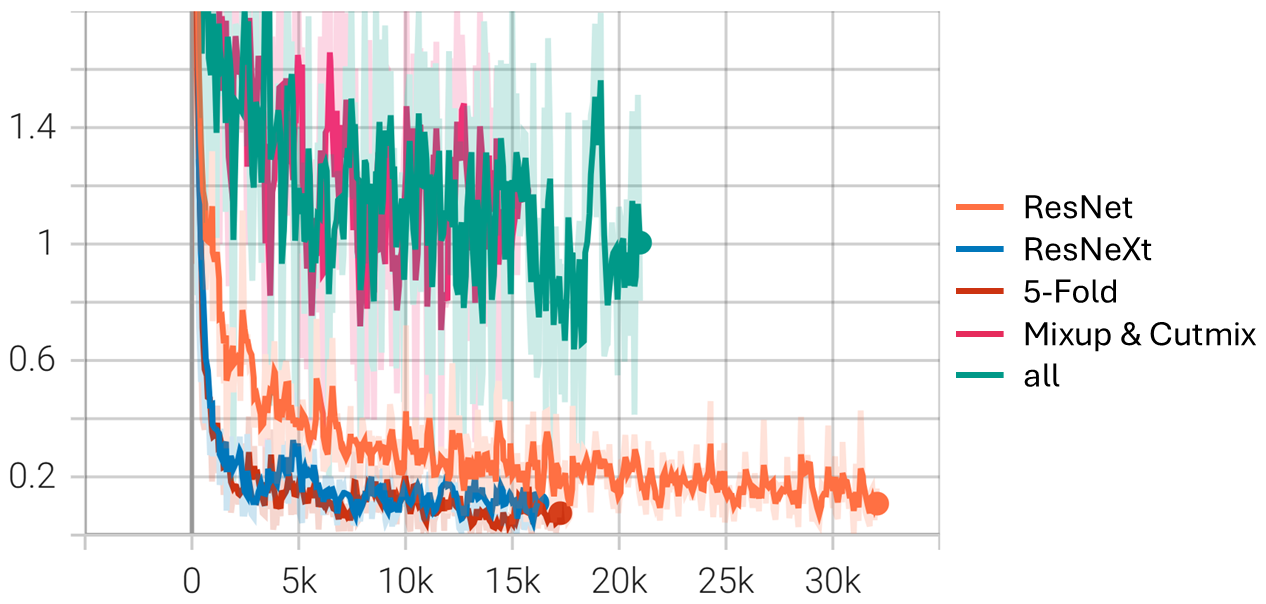
\includegraphics[width=0.9\linewidth]{assets/train_loss.png}
  \caption{\textbf{Training loss curve.} Only a single sub-model is selected
    for 5-Fold and All to better visualize.}
  \label{fig:train-loss}
\end{figure}

\begin{figure}[h]
  \centering
  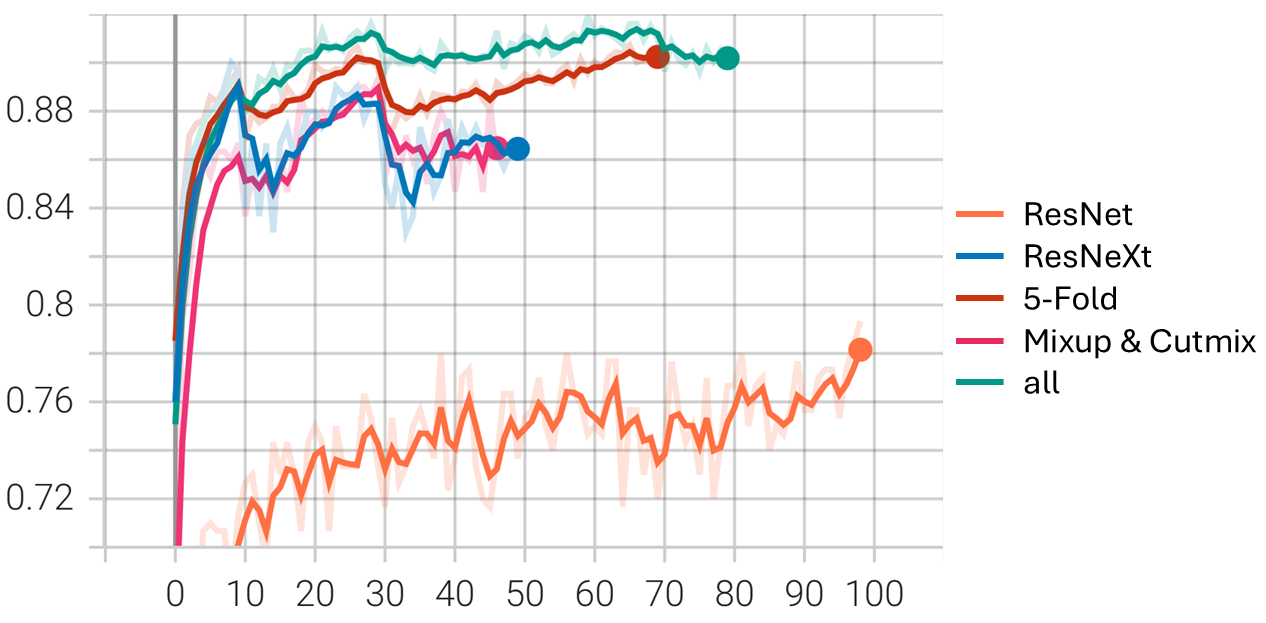
\includegraphics[width=0.9\linewidth]{assets/val_acc.png}\
  \caption{\textbf{Validation accuracy curve.} The selection of those two curve
    is the same as \cref{fig:train-loss}.}
  \label{fig:val-acc}
\end{figure}

\section*{Other Experiments}

\subsection*{The Selection of Backbone}

The selection of the backbone is crucial for the model's performance. I've
conducted experiments with different backbones, including a variant of ResNet,
ResNeXt and ResNeSt~\cite{zhang2020resnest}. The results are shown in
\cref{fig:exp-backbone-acc}. While ResNeSt achieves the highest validation
accuracy, it performs poorly on the test set. ResNeXt is the most stable
backbone, with consistent performance across all datasets. Therefore, I choose
ResNeXt as the backbone for the following experiments.

\begin{figure}[h]
  \centering
  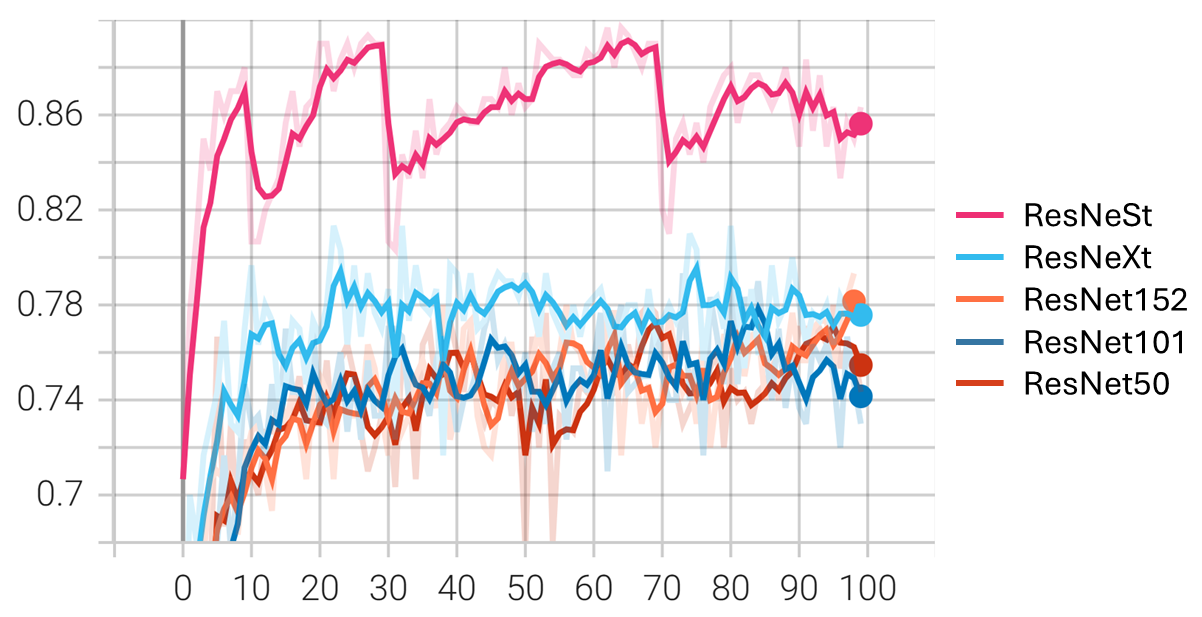
\includegraphics[width=0.9\linewidth]{assets/exp_backbone_acc.png}
  \caption{\textbf{Validation accuracy of different backbones.} The results are
    evaluated by choosing the best checkpoint based on the validation accuracy.}
  \label{fig:exp-backbone-acc}
\end{figure}

I've also experimented with different tricks, such as focal loss~\cite{FocalLoss2017}
, image normalization (normalize the image before feeding into the model), trivial
data augmentation, and random data augmentation~\cite{PyTorch_aug}.
All these experiments are based on the backbone, ResNeXt. The results
are shown in \cref{tab:tricks}. However, none of these
tricks improve the model's performance. Therefore, they are not included in
the final model.

\begin{table}[h]
  \centering
  \begin{tabular}{lccc}
    \toprule
    \multicolumn{1}{c}{\textbf{Trick}} & \textbf{Val}                   & \textbf{Test pub.}             & \textbf{Test priv.}            \\
    \midrule
    Backbone                           & 0.9000                         & 0.9317                         & 0.9266                         \\
    \hdashline
    Focal loss                         & \cellcolor[HTML]{FFCCC9}0.8933 & \cellcolor[HTML]{CBDBFF}0.9326 & \cellcolor[HTML]{FFCCC9}0.9104 \\
    Normalization                      & \cellcolor[HTML]{FFCCC9}0.8833 & \cellcolor[HTML]{FFCCC9}0.9138 & \cellcolor[HTML]{FFCCC9}0.9078 \\
    Random Aug.                        & \cellcolor[HTML]{FFCCC9}0.8933 & \cellcolor[HTML]{FFCCC9}0.9215 & \cellcolor[HTML]{FFCCC9}0.9078 \\
    Trivial Aug.                       & \cellcolor[HTML]{CBDBFF}0.9033 & \cellcolor[HTML]{CBDBFF}0.9326 & \cellcolor[HTML]{CBDBFF}0.9317 \\
    \bottomrule
  \end{tabular}
  \caption{\textbf{Accuracy results of different tricks.} The red background
    indicates a decrease in accuracy, while the blue one indicates an increase.}
  \label{tab:tricks}
\end{table}

Also, different strategies for combining test-time ensemble are tested. It
includes output average, output probability average (softmax), and majority
vote. The results are shown in \cref{tab:ensemble}. The output
average achieves the best performance, so it is used in the final model.

\begin{table}[h]
  \centering
  \begin{tabular}{lcc}
  \toprule
  \multicolumn{1}{c}{\textbf{Trick}} & \textbf{Test pub.} & \textbf{Test priv.} \\
  \midrule
  Average                            & \textbf{0.9522}    & \textbf{0.9514}     \\
  Softmax avg.                       & 0.9514             & 0.9480              \\
  Vote                               & 0.9480             & 0.9445              \\
  Single sub-model                   & 0.9420             & 0.9300              \\
  \bottomrule
  \end{tabular}
  \caption{\textbf{Accuracy results of different ensemble strategies.} The bold 
    words indicate the best performance.}
  \label{tab:ensemble}
\end{table}

%%%%%%%%% REFERENCES %%%%%%%%%
{\small
\bibliographystyle{ieee_fullname}
\bibliography{egbib}
}

\end{document}